In this chapter we present comparisons between seismic hazard results computed using OpenQuake and alternative software for real national/regional scale seismic hazard models. We present three cases: the seismic hazard model for the 2005 national building code of Canada (\cite{adams2003}, \cite{halchuk2008}), the 2008 U.S. national seismic hazard model (\cite{petersen2008}), and the 2012 national seismic hazard model for Australia (\cite{burbidge2012}). We refer the reader to the original reports for an in-depth description of each model. Here we present only the main features and the aspects of interest for the software implementation.


\section{The national seismic hazard model for the 2005 building code of Canada}

\subsection{The seismic source model}
To capture epistemic uncertainties in the seismic source definiton, two complete seismic source models are defined: the historical (\textbf{H}) and regional (\textbf{R}) models. The historical model uses relatively small source zones drawn around historical seismicity clusters, while the regional model defines larger, regional zones reflecting seismotectonic units. Both models are composed of area sources, with the only exception of the Queen Charlotte fault (in western Canada) treated as a fault source. Occurrence rates in each source are defined through a double-truncated Gutenberg-Richter distribution, with minimum magnitude equal to 4.75.
Epistemic uncertainties in the magnitude-frequency distribution are captured by the definition for each source of three possible ($a_{GR}$, $b_{GR}$) pairs and three possible maximum magnitudes. Each source is also associated to three possible hypocentral depths. The model prescribes also a floor model (\textbf{F}) for the relatively aseismic central part of Canada and a deterministic model for the Cascadia subdution zone (\textbf{C}).\\
Earthquake ruptures associated with area sources are assumed to have no spatial extension (that is point ruptures), while earthquakes on faults follow a magnitude-length scaling relationship ($L=10^{-1.085 + 0.389 m}$)

\subsection{The ground motion model}
The ground motion model distinguishes between eastern and western Canada because of the different properties in the crust. For eastern and central Canada the GMPE model of \cite{ab1995} is used. For western Canada the model of \cite{bjf1993} is used for shallow crustal sources, while for deep intraslab sources the model of \cite{y1997} is adopted. Epistemic uncertainties are included by defining, for each GMPE, a pair of parallel alternative relations, with higher and lower mean values.

\subsection{Reference site conditions}
Hazard maps are computed for a \textit{reference} ground condition corresponding to "Site Class C" (firm-ground), defined by a 360 to 750 m/s $Vs_{30}$. For central and eastern Canada, hazard map values computed with the hard-rock GMPE of \cite{ab1995} are adjusted for firm-ground. That is, seismic hazard spectral values are amplified by a period-dependent 'reference ground condition' factor (see Table 2 in \cite{adams2003}). For western canada, the model of \cite{y1997} is adjusted for firm-ground. The model of \cite{bjf1993} does not require instead any adjustment given that its "Soil Class B" is identical to "Site Class C".

\subsection{Implementation of the model in the OpenQuake-engine}
Currently, only the \textbf{H} and \textbf{R} models are implemented in the Openquake-engine. We set the discretization step for area sources to 5 km, and model ruptures as points. The discretization step for the Queen Charlotte fault is instead 2 km, and the rupture extension is modeled using the magnitude-area scaling relationship of \cite{wells1994}. The OpenQuake-engine does not currently support the inclusion of magnitude-length scaling relationships and this prevent us from exactly reproducing the original rupture modeling for the Queen Charlotte fault. \\
For each source in both the \textbf{H} and \textbf{R} model, we computed a mean magnitude-frequency distribution by considering all possible (that is 9) ($a_{GR}$, $b_{GR}$) - $M_{max}$ combinations. That is, for each magnitude bin (of 0.1 magnitude units width), we defined the occurrence rate as the weighted mean of the rates obtained from the different possible magnitude-frequency distributions.\\
For each site, contributions from ruptures that are within a radius of 600 km are considered for the central and eastern Canada models and of 400 km for the western Canada models (consistently to what done by \cite{adams2003}). The original calculation assumes the ground motion distribution to be untruncated. To reproduce such condition, we assume in the OpenQuake-engine calculation a truncation level equal to 6 sigmas.

\subsection{Comparison against Canada hazard maps}
We compare the OpenQuake-engine results against hazard maps obtained from \textit{mean} hazard curves produced by the Geological Survey of Canada (GSC) using a modified version of the commercial software FRISK88 (http://www.riskeng.com/software/frisk88m/). The GSC approach for constructing hazard maps (for a given probability of exceedance or return period) relies on the so-called 'robust' method (\cite{adams2003}). The method is based on choosing, from the four models (\textbf{H}, \textbf{R}, \textbf{F} and \textbf{C}), the highest value for each grid point accross Canada. Using the OpenQuake-engine we thus computed hazard map values for the sites accross Canada for which the \textbf{H} or \textbf{R} models give the highest values. A comparison for the $10\%$ probability of exceedance map for PGA is shown in Figure \ref{fig:canada_475y_hmaps}.
\begin{figure}
\centering
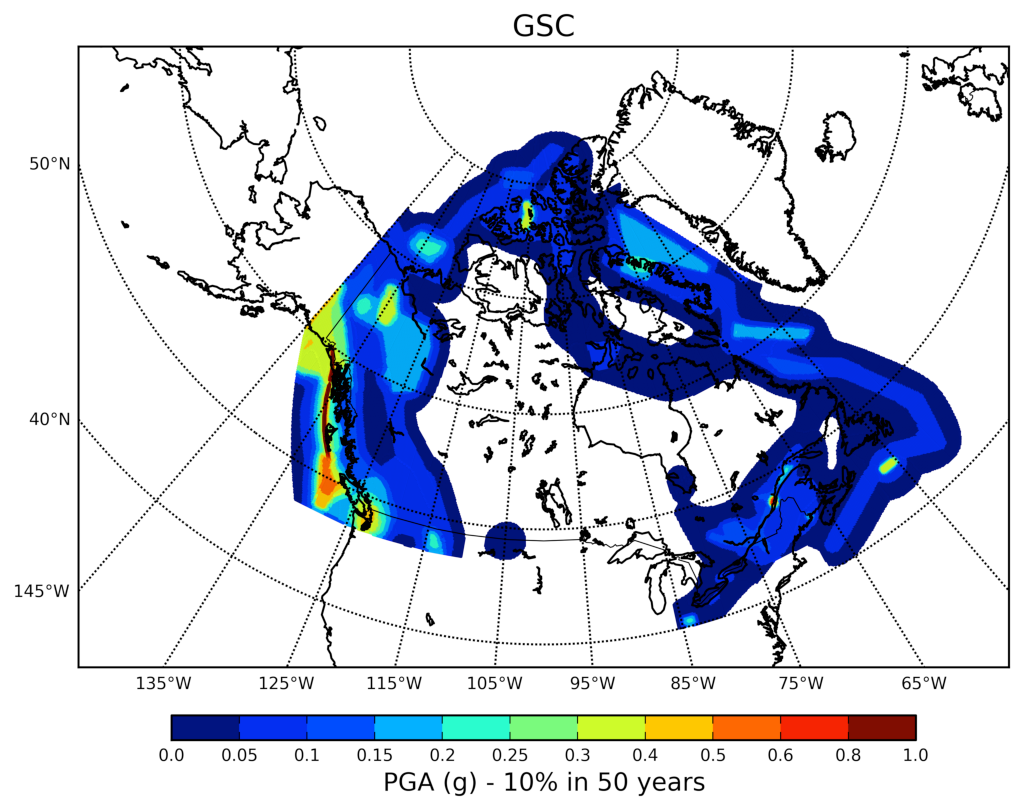
\includegraphics[width=14cm]{./qareport/pictures/GSC_combined_PGA_0pt1_firm_ground.pdf}
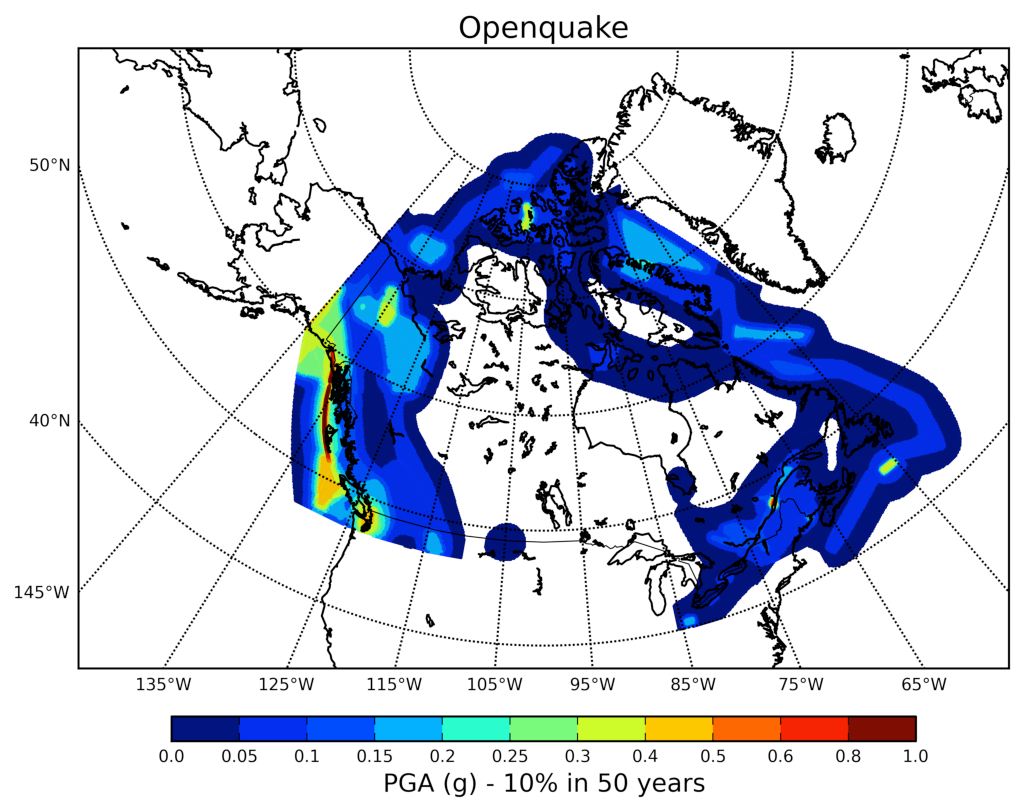
\includegraphics[width=14cm]{./qareport/pictures/OQ_combined_PGA_0pt1_firm_ground.pdf}
\caption{Official hazard map produced by the Geological Survey of Canada (top) and by the OpenQuake-engine implementation (bottom)}
\label{fig:canada_475y_hmaps}
\end{figure}
\begin{figure}
\centering
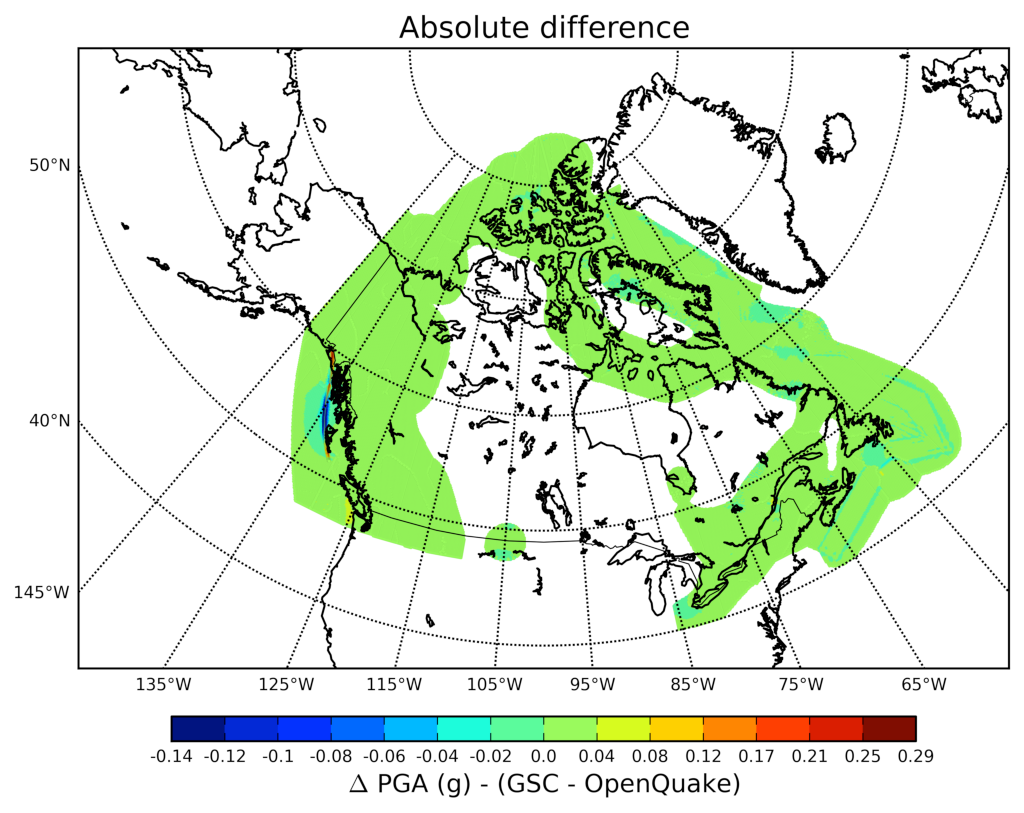
\includegraphics[width=14cm]{./qareport/pictures/GSC_OQ_PGA_0pt1_abs_diff.pdf}
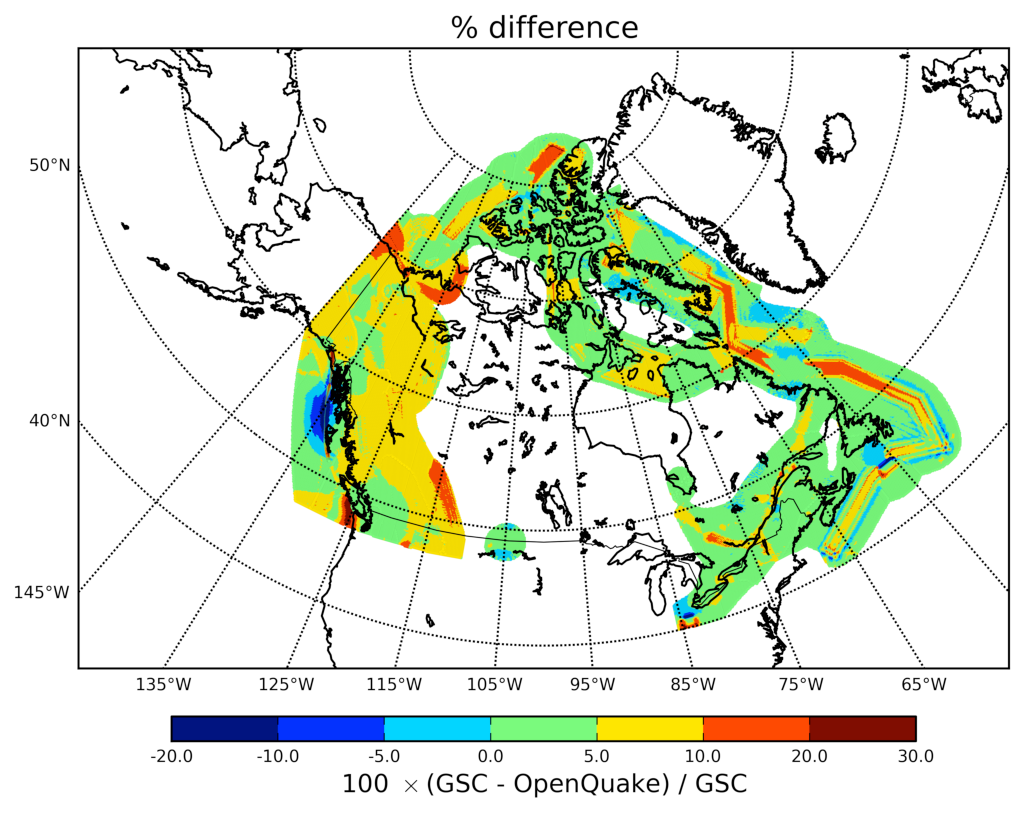
\includegraphics[width=14cm]{./qareport/pictures/GSC_OQ_PGA_0pt1_percent_diff.pdf}
\caption{Absolute (top) and percent (bottom) difference maps between the official GSC hazard map and the one produced by the OpenQuake-engine as visible in Figure \ref{fig:canada_475y_hmaps}}
\label{fig:canada_475y_dmaps}
\end{figure}
The comparison between the hazard maps reveals a satisfactory agreement, at least from a visual perspective. Difference maps (Figure \ref{fig:canada_475y_dmaps}) are however more informative and provide a quantitative understanding of the differences between the two maps. The absolute difference map shows that for the vast majority of the grid points, the GSC solution over-estimates the OpenQuake-engine solution by values between 0 and 0.04 g. The highest positive differences (GSC > OpenQuake-engine), up to 0.3 g, are instead only visible along the Queen Charlotte fault, especially at the north and south endings of the fault trace. The highest negative differences (GSC < OpenQuake-engine) are still along the Queen Charlotte fault, especially in the region close to the middle part of the fault trace. These differences can be reasonably motivated by the previously mentioned fact that, for the Queen Charlotte fault, we cannot use in the OpenQuake-engine a magnitude-length scaling relationship as originally defined by the model. We thus used the \cite{wells1994} magnitude-area scaling relationship. The discrepancies reflect not only different functional forms but also different ways of defining ruptures' size and shape. Indeed when using a magnitude-length scaling relationship, no rupture reshaping (for area conservation) is required which is instead a key feature when considering a magnitude-area scaling law. The relative percent error shows instead the significance of the absolute difference in the various regions covered by the hazard map. Percent differences ranges from $-20\%$ to $30\%$. The highest positive differences are visible along the area sources associated with low hazard values. Some significant differences are visible along the boundaries of rectangular zones such as the small rectangular area source close to the village of Anna, in Ohio, U.S. (85W, 40N) and the source south of the Newfoundland, Canada (approximately 60W, 45N). Inside those sources the hazard levels are relatively high (between 0.15 and 0.2 g for the former and between 0.3 and 0.4 for the latter). Within the boundary the relative error is less than $5\%$. The larger differences along the boundary may be therefore the effect of different discretization algorithms in the two software.